\documentclass{report}
\usepackage{graphicx, tikz-cd, float, titlepic, booktabs} % Required for inserting images
\usepackage{pgfplots}
\pgfplotsset{compat=1.15}
\usepackage{mathrsfs}
\usetikzlibrary{arrows}
\usepackage{amsmath, amssymb, amsthm, amsfonts, siunitx, physics, gensymb}
\AtBeginDocument{\RenewCommandCopy\qty\SI}
\usepackage[version=4]{mhchem}
\usepackage[most,many,breakable]{tcolorbox}
\usepackage{xcolor, fancyhdr, varwidth}
\usepackage[Glenn]{fncychap}
%Options: Sonny, Lenny, Glenn, Conny, Rejne, Bjarne, Bjornstrup
\usepackage{hyperref, cleveref}
\usepackage{icomma, enumitem} %comma as decimal and continue enumerate with [resume]
\usepackage[danish]{babel}
%%%%%%%%%%%%%%%%%%%%%%%%%%%%%%
% SELF MADE COLORS
%%%%%%%%%%%%%%%%%%%%%%%%%%%%%%
\definecolor{myg}{RGB}{56, 140, 70}
\definecolor{myb}{RGB}{45, 111, 177}
\definecolor{myr}{RGB}{199, 68, 64}
\definecolor{mytheorembg}{HTML}{F2F2F9}
\definecolor{mytheoremfr}{HTML}{00007B}
\definecolor{mylenmabg}{HTML}{FFFAF8}
\definecolor{mylenmafr}{HTML}{983b0f}
\definecolor{mypropbg}{HTML}{f2fbfc}
\definecolor{mypropfr}{HTML}{191971}
\definecolor{myexamplebg}{HTML}{F2FBF8}
\definecolor{myexamplefr}{HTML}{88D6D1}
\definecolor{myexampleti}{HTML}{2A7F7F}
\definecolor{mydefinitbg}{HTML}{E5E5FF}
\definecolor{mydefinitfr}{HTML}{3F3FA3}
\definecolor{notesgreen}{RGB}{0,162,0}
\definecolor{myp}{RGB}{197, 92, 212}
\definecolor{mygr}{HTML}{2C3338}
\definecolor{myred}{RGB}{127,0,0}
\definecolor{myyellow}{RGB}{169,121,69}
\definecolor{myexercisebg}{HTML}{F2FBF8}
\definecolor{myexercisefg}{HTML}{88D6D1}
%%%%%%%%%%%%%%%%%%%%%%%%%%%%%%%%%%%%%%%%%%%%%%%%%%%%%%%%%%%%%%%%%%%%%%
% Box environments for theorems and problems
%%%%%%%%%%%%%%%%%%%%%%%%%%%%%%%%%%%%%%%%%%%%%%%%%%%%%%%%%%%%%%%%%%%%%
\setlength{\parindent}{1cm}
%================================
% Question BOX
%================================
\makeatletter
\newtcbtheorem{question}{Opgave}{enhanced,
	breakable,
	colback=white,
	colframe=myb!80!black,
	attach boxed title to top left={yshift*=-\tcboxedtitleheight},
	fonttitle=\bfseries,
	title={#2},
	boxed title size=title,
	boxed title style={%
			sharp corners,
			rounded corners=northwest,
			colback=tcbcolframe,
			boxrule=0pt,
		},
	underlay boxed title={%
			\path[fill=tcbcolframe] (title.south west)--(title.south east)
			to[out=0, in=180] ([xshift=5mm]title.east)--
			(title.center-|frame.east)
			[rounded corners=\kvtcb@arc] |-
			(frame.north) -| cycle;
		},
	#1
}{def}
\makeatother
%================================
% DEFINITION BOX
%================================

\newtcbtheorem[]{Definition}{Definition}{enhanced,
	before skip=2mm,after skip=2mm, colback=red!5,colframe=red!80!black,boxrule=0.5mm,
	attach boxed title to top left={xshift=1cm,yshift*=1mm-\tcboxedtitleheight}, varwidth boxed title*=-3cm,
	boxed title style={frame code={
					\path[fill=tcbcolback]
					([yshift=-1mm,xshift=-1mm]frame.north west)
					arc[start angle=0,end angle=180,radius=1mm]
					([yshift=-1mm,xshift=1mm]frame.north east)
					arc[start angle=180,end angle=0,radius=1mm];
					\path[left color=tcbcolback!60!black,right color=tcbcolback!60!black,
						middle color=tcbcolback!80!black]
					([xshift=-2mm]frame.north west) -- ([xshift=2mm]frame.north east)
					[rounded corners=1mm]-- ([xshift=1mm,yshift=-1mm]frame.north east)
					-- (frame.south east) -- (frame.south west)
					-- ([xshift=-1mm,yshift=-1mm]frame.north west)
					[sharp corners]-- cycle;
				},interior engine=empty,
		},
	fonttitle=\bfseries,
	title={#2},#1}{def}
\newtcbtheorem[]{definition}{Definition}{enhanced,
	before skip=2mm,after skip=2mm, colback=red!5,colframe=red!80!black,boxrule=0.5mm,
	attach boxed title to top left={xshift=1cm,yshift*=1mm-\tcboxedtitleheight}, varwidth boxed title*=-3cm,
	boxed title style={frame code={
					\path[fill=tcbcolback]
					([yshift=-1mm,xshift=-1mm]frame.north west)
					arc[start angle=0,end angle=180,radius=1mm]
					([yshift=-1mm,xshift=1mm]frame.north east)
					arc[start angle=180,end angle=0,radius=1mm];
					\path[left color=tcbcolback!60!black,right color=tcbcolback!60!black,
						middle color=tcbcolback!80!black]
					([xshift=-2mm]frame.north west) -- ([xshift=2mm]frame.north east)
					[rounded corners=1mm]-- ([xshift=1mm,yshift=-1mm]frame.north east)
					-- (frame.south east) -- (frame.south west)
					-- ([xshift=-1mm,yshift=-1mm]frame.north west)
					[sharp corners]-- cycle;
				},interior engine=empty,
		},
	fonttitle=\bfseries,
	title={#2},#1}{def}

\newtcbtheorem{theo}%
    {Theorem}{}{theorem}
\newtcolorbox{prob}[1]{colback=red!5!white,colframe=red!50!black,fonttitle=\bfseries,title={#1}}
%================================
% NOTE BOX
%================================

\usetikzlibrary{arrows,calc,shadows.blur}
\tcbuselibrary{skins}
\newtcolorbox{note}[1][]{%
	enhanced jigsaw,
	colback=gray!20!white,%
	colframe=gray!80!black,
	size=small,
	boxrule=1pt,
	title=\textbf{Note:},
	halign title=flush center,
	coltitle=black,
	breakable,
	drop shadow=black!50!white,
	attach boxed title to top left={xshift=1cm,yshift=-\tcboxedtitleheight/2,yshifttext=-\tcboxedtitleheight/2},
	minipage boxed title=1.5cm,
	boxed title style={%
			colback=white,
			size=fbox,
			boxrule=1pt,
			boxsep=2pt,
			underlay={%
					\coordinate (dotA) at ($(interior.west) + (-0.5pt,0)$);
					\coordinate (dotB) at ($(interior.east) + (0.5pt,0)$);
					\begin{scope}
						\clip (interior.north west) rectangle ([xshift=3ex]interior.east);
						\filldraw [white, blur shadow={shadow opacity=60, shadow yshift=-.75ex}, rounded corners=2pt] (interior.north west) rectangle (interior.south east);
					\end{scope}
					\begin{scope}[gray!80!black]
						\fill (dotA) circle (2pt);
						\fill (dotB) circle (2pt);
					\end{scope}
				},
		},
	#1,
}
%================================
% EXAMPLE BOX
%================================
\newtcbtheorem[number within=section]{Example}{Example}
{%
	colback = myexamplebg
	,breakable
	,colframe = myexamplefr
	,coltitle = myexampleti
	,boxrule = 1pt
	,sharp corners
	,detach title
	,before upper=\tcbtitle\par\smallskip
	,fonttitle = \bfseries
	,description font = \mdseries
	,separator sign none
	,description delimiters parenthesis
}
{ex}
%================================
% THEOREM BOX
%================================

\tcbuselibrary{theorems,skins,hooks}
\newtcbtheorem[number within=section]{Theorem}{Theorem}
{%
	enhanced,
	breakable,
	colback = mytheorembg,
	frame hidden,
	boxrule = 0sp,
	borderline west = {2pt}{0pt}{mytheoremfr},
	sharp corners,
	detach title,
	before upper = \tcbtitle\par\smallskip,
	coltitle = mytheoremfr,
	fonttitle = \bfseries\sffamily,
	description font = \mdseries,
	separator sign none,
	segmentation style={solid, mytheoremfr},
}
{th}

%%%%%%%%%%%%%%%%%%%%%%%%%%%%%%%%%%%%%%%%%%%%%%%%%%%%%%%%%%%%%%%%%
% SELF MADE COMMANDS
%%%%%%%%%%%%%%%%%%%%%%%%%%%%%%
\newcommand{\sol}{\setlength{\parindent}{0cm}\textbf{\textit{Løsning:}}\setlength{\parindent}{1cm}}
%%%%%%%%%%%%%%%%%%%%%%%%%%%%%%%%%
\usepackage[tmargin=2cm,rmargin=1in,lmargin=1in,margin=0.85in,bmargin=2cm,footskip=.2in]{geometry}\pagestyle{fancy}
\lhead{Minrui Kevin Zhou 3.b}
\rhead{H1: Mekanik}

\title{Hjemmeopgave H1: Mekanik\\
{\Large \textbf{3.b fys A}}}
\author{Kevin Zhou}
\date{\today}

\begin{document}
\maketitle
\begin{question}{Månehop}{}
  Fotoet stammer fra en filmoptagelse af en astronauts hop på overfladen af Månen. Tabellen viser sammenhørende værdier af tiden og astronautens lodrette hastighed $v$ under hoppet. Til $t=0 \;\unit{s} $ slipper astronautens fødder måneoverfladen. Astronauten hoppede med strakt krop.
\begin{itemize}
  \item[a.] Bestem ud fra tabellens data en værdi for tyngdeaccelerationen på Månen.
  \item[b.] Bestem ud fra tabellens data, til hvilket tidspunkt astronauten befandt sig øverst i hoppet. Hvor højt hoppede astronauten?
\end{itemize}
\end{question}
\sol \\
\textbf{a.}
Vi har med uafhængighedsprincippet
\[
v_{y}=-g \cdot t + v_{0y} 
\]
Denne kan opfattes som en linæer funktion af $t$.
Tabellens data ses i \cref{fig:astronaut}.
\begin{figure}[H]
\begin{center}
  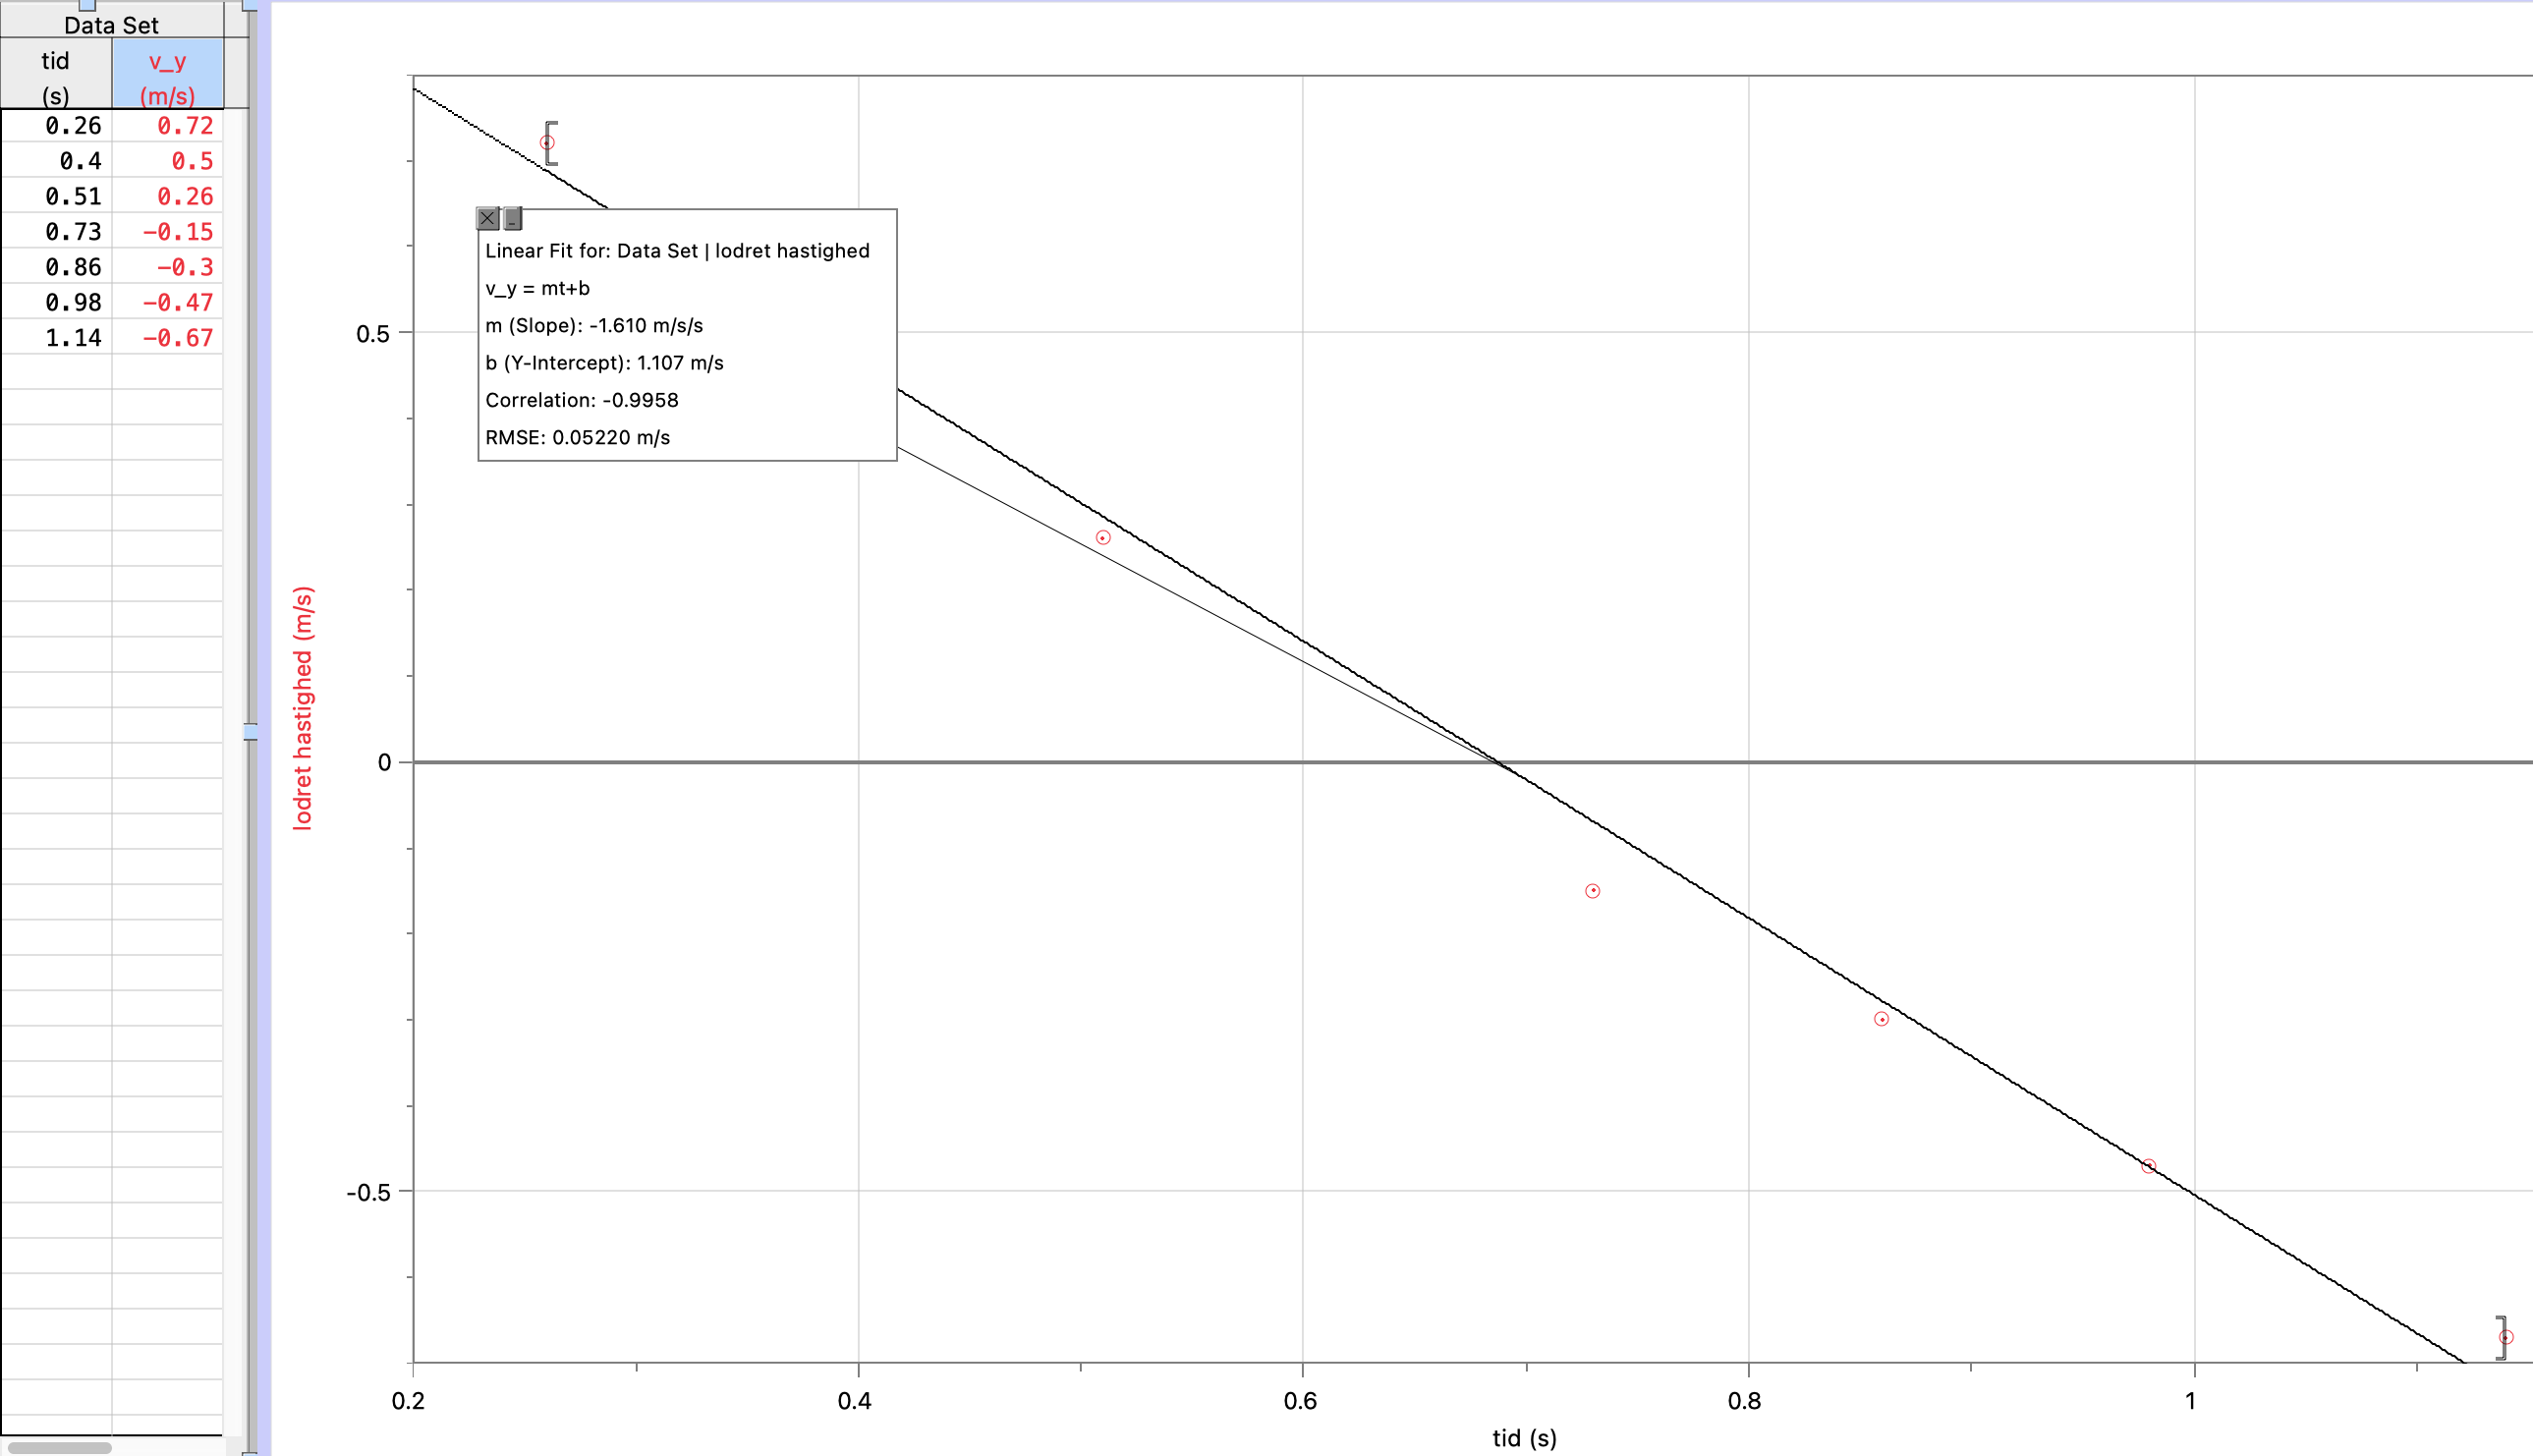
\includegraphics[scale=0.3]{astronaut.png}
\end{center}
\caption{Lineær regression af tabellens data}
\label{fig:astronaut}
\end{figure}
Hældningen af $(t,v)$-grafen er da $-g$.
Fra denne ser vi, at tyngdeaccelerationen er 
\begin{equation*}
\begin{split}
  g&=-(-1,610 \;\unit{m/s^2} )\\ 
  &\approx 1,6 \;\unit{m/s^2} 
\end{split}
\end{equation*}
Altså er tyngdeaccelerationen på månen $1,6 \;\unit{m/s^2} $.\\[1ex]
\textbf{b.}
Vi har, at 
\begin{equation*}
\begin{split}
  t_{\text{top} }&=\frac{v_{0y}}{g}\\ 
  &=\frac{1,107 \;\unit{m/s} }{1,610 \;\unit{m/s^2} }\\ 
  &=0,68758 \;\unit{s} \\ 
  &\approx 0,69 \;\unit{s} 
\end{split}
\end{equation*}
Nu kan vi regne hoppets højde ud.
\begin{equation*}
\begin{split}
  y_{\text{max} }&=v_{0y} \cdot t_{\text{top} } - \frac{1}{2}\cdot g \cdot t_{\text{top} }^2\\ 
  &=1,107 \;\unit{m/s} \cdot 0,68758 \;\unit{s} - \frac{1}{2} \cdot 1,610 \;\unit{m/s^2} \cdot \left(0,68758 \;\unit{s} \right)^2 \\ 
  &\approx 0,38 \;\unit{m} 
\end{split}
\end{equation*}
Astronauten befandt sig altså øverst i hoppet efter $0,69 \;\unit{s} $ og hoppede $0,38 \;\unit{m} $ højt. 
\begin{question}{Målspark}{}
Under en fodboldkamp diskuterer to tilskuere, hvilken fart fodbolden opnår ved et målspark. De beslutter at vurdere denne fart ved det næste målspark. Den ene tilskuer måler, at der går $2,9 \;\unit{s} $, fra fodbolden forlader målmandens fod, til fodbolden igen rammer jorden. Den anden tilskuer bestemmer den vandrette afstand mellem fodboldens startsted og nedslagssted til $60 \;\unit{m} $.
\begin{itemize}
  \item[a.] Beregn fodboldens middelhastighed i vandret retning.
\end{itemize}

Man kan få en mere nøjagtig værdi for den søgte begyndelsesfart ved også at tage hensyn til fodboldens bevægelse i lodret retning.
\begin{itemize}
  \item[b.] Bestem en mere nøjagtig værdi for fodboldens begyndelsesfart. Man kan se bort fra luftmodstanden.
\end{itemize}
\end{question}
\sol \\
\textbf{a.}
Middelhastigheden i vandret retning er
\begin{equation*}
\begin{split}
  v_{\text{vandret} }&=\frac{\Delta s}{\Delta t}\\ 
  &=\frac{60 \;\unit{m} }{2,9 \;\unit{s} }\\ 
  &\approx 21 \;\unit{m/s} 
\end{split}
\end{equation*}
Altså er fodboldens middelhastighed i vandret retning $21 \;\unit{m/s} $.\\[1ex]
\textbf{b.}
Vi har, at
\[
t_{\text{top} }=\frac{2,9 \;\unit{s} }{2}=\frac{v_0 \cdot \sin\left(\theta\right) }{g} &\implies v_0= \frac{g \cdot 1,45 \;\unit{s} }{\sin\left(\theta\right) }
\] 
Der gælder også, at 
\begin{equation*}
\begin{split}
x_{\text{max} }=v_0 \cdot \cos\left(\theta\right) \cdot t_{\text{kast} } &\implies 60 \;\unit{m} =\frac{g \cdot 1,45 \;\unit{s} \cdot \cos\left(\theta\right) \cdot 2,9 \;\unit{s} }{\sin\left(\theta\right) }\\ 
&\iff 60=41,209 \cdot \cot(\theta)\\ 
  &\iff  \theta = \pi n + \cot^{-1}\left(\frac{60}{41,209}\right), \quad n \in \mathbb{Z}
\end{split}
\end{equation*}
Bemærk, at er flere forskellige vinkler, der er løsninger.
Vi regner nu $v_0$.
\begin{equation*}
\begin{split}
  v_0&=\frac{g \cdot 1,45 \;\unit{s} }{\sin\left(\theta\right) }\\ 
  &=\frac{9,8 \;\unit{m/s^2} \cdot 1,45 \;\unit{s} }{\sin\left(\pi n + \cot^{-1}\left(\frac{60}{41,209}\right)\right) }, \quad n \in \mathbb{Z}\\ 
  &\approx \pm 25 \;\unit{m/s} 
\end{split}
\end{equation*}
Da begyndelsesfarten jo kun kan være positiv, så er en mere nøjagtig værdi for denne, når man ser bort fra luftmodstanden, $25 \;\unit{m/s} $.
\begin{question}{Dart}{}
  I spillet dart kaster spillerne små pile mod en skive, som er inddelt i pointfelter. Man får
  flest point ved at ramme bull's-eye, der er et lille cirkelformet område midt på skiven.
  En dartspiller kaster en pil. Herunder accelererer han med en hurtig håndbevægelse pilen fra hvile op til farten $5,9 \;\unit{m/s}$ i løbet af $0,12 \;\unit{s} $.
\begin{itemize}
  \item[a.] Beregn størrelsen af pilens gennemsnitlige acceleration.
\end{itemize}
Dartspilleren forsøger at ramme bull's-eye og sigter derfor mod et punkt lidt over skivens centrum. Han sender pilen af sted skråt opad med farten $5,9 \;\unit{m/s}$ og i en vinkel på $18,6 \degree $ med vandret. Pilen slippes $2,21 \;\unit{m} $ fra skiven i samme højde over gulvet som skivens centrum. Bull's-eye har diameteren $12,7 \;\unit{mm}$.
\begin{itemize}
  \item[b.] Vurdér, om pilen rammer bull's-eye.
\end{itemize}
\end{question}
\sol \\
Det er værd at tilføje, at feltet, der giver flest point i dart, modsat det, der står i opgaven, faktisk er triple 20, der giver 60 point, og ikke bull's-eye, der kun giver 50.\\[1ex]
\textbf{a.}
Størrelsen af den gennemsnitlige acceleration er 
\begin{equation*}
\begin{split}
  \abs{\va{a} _{\text{middel} }}&=\frac{\Delta \abs{\va{v}}}{\Delta t}\\ 
  &=\frac{5,9 \;\unit{m/s} -0 \;\unit{m/s} }{0,12 \;\unit{s} }\\ 
  &\approx 49 \;\unit{m/s^2} 
\end{split}
\end{equation*}
Altså er størrelsen af pilens gennemsnitlige acceleration $49 \;\unit{m/s^2} $.\\[1ex]
\textbf{b.}
For at finde ud af, om pilen rammer bull's-eye, sætter vi blot de kendte værdier ind i ligningen for banekurven for et skråt kast og ser, om det er sandt, at $y \in [6,35;-6,35] \;\unit{mm} $ (fordi bull's-eye jo har radius på $\frac{12,7}{2}\;\unit{mm}$).
\begin{equation*}
\begin{split}
  y&=-\frac{g}{2 \cdot v_0^2 \cdot \cos^2\left(\theta\right) }\cdot x^2 + \tan\left(\theta\right) \cdot x\\ 
  &=-\frac{9,8 \;\unit{m/s^2} }{2 \cdot \left(5,9 \;\unit{m/s} \right)^2 \cdot \cos^2\left(18,6 \degree \right) }\cdot \left(2,21 \;\unit{m} \right)^2 + \tan\left(18,6 \degree \right) \cdot 2,21 \;\unit{m} \\ 
  &\approx -0,022 \;\unit{m} \\ 
  &=22 \;\unit{mm} \not\in [6,35\;\unit{mm};-6,35\;\unit{mm}]  
\end{split}
\end{equation*}
Altså rammer pilen ikke bull's-eye.
\end{document}
